\begin{document}
\title{COMS3008A Assignment -- Report}
\author{Sahil Dinanath, Darshan Singh}
\date{Put your submission date here} 
\maketitle 
%\thispagestyle{empty}
\pagestyle{fancy}
\fancyhf{}
\fancyhead[R]{\thepage}
\fancyhead[L]{COMS3008A Assinment}
%\vskip 3mm 
%\pagenumbering{roman}
%\newpage
\pagenumbering{arabic} 
\section{Problem 1: Parallel Scan}
\begin{itemize}
	\item  Given a set of elements, $[a_0,a_1,\dotsm,a_{n-1}]$, the scan operation associated with addition operator for this input is the output set $[a_0,(a_0+a_1),\dotsm,(a_0+a_1+\dotsm+a_{n-1})]$. 
	\item For example, the input set is $[2,1,4,0,3,7,6,3]$, then the scan with addition operator of this input is $[2,3,7,7,10,17,23,26]$. 
\end{itemize}
\subsection*{Approach}
\subsection{Serial} 
\subsection{OpenMP} 
\subsection{MPI}
\pagebreak
\section{Problem 2: Parallel Bitonic Sort}
\subsection*{Approach}
\subsection{Serial} 
\subsubsection{Algorithm}
The main code that implements the Bitonic Sort algorithm is shown in Listing \ref{lst:bitonic_sort}.

\begin{lstlisting}[language=C, caption={Bitonic Sort Algorithm}, label={lst:bitonic_sort}]
// Code snippet of the Bitonic Sort algorithm
// Function definitions for compAndSwap, bitonicMerge, and bitonicSort

int main(int argc, char *argv[]) {
  // Initialization and setup code
  // Read input file and convert characters to integers
  // Start timing
  // Call bitonicSort to sort the input array
  // Stop timing
  // Print sorted array
}
\end{lstlisting}

\subsubsection{Testing}
The code begins by reading the input file and converting the characters to integers. This section of the code consists of the following functions:

\begin{itemize}
  \item \texttt{getFileSize}: This function determines the size of the input file by seeking to the end of the file, retrieving the current position (which represents the file size), and then resetting the file position to the beginning.
  \item \texttt{readFile}: This function reads the contents of the input file into a character array \texttt{line} using the \texttt{fgets} function. It also closes the file after reading.
  \item \texttt{convertCharToIntArray}: This function converts the character array \texttt{fileCharacters} into an array of long integers \texttt{input} by subtracting the ASCII value of \texttt{'0'} from each character.
\end{itemize}

\subsubsection{Results}
The Bitonic Sort algorithm is then applied to the input array using the \texttt{bitonicSort} function. The execution time of the sorting process is measured using the \texttt{omp\_get\_wtime} function. Finally, the sorted array is printed using the \texttt{printArray} function, and the total execution time is displayed.
\begin{table}[htb]
	\centering
	\caption{Bitonic sort with different input sizes}\label{tab:example}
	\begin{tabular}{l|ccccc}
		\toprule
		No of characters & $2^3$ & $2^{16}$ & $2^{23}$ & $2^{26}$ & $2^{28}$\\
		\midrule
		Serial &0.1&0.2&0.3&0.4&0.5\\
		Parallel &&&&\\
		Speedup &2&3&4&5&6\\
		\bottomrule
	\end{tabular}
\end{table} 
\subsection{OpenMP} 
\subsection{MPI}
\pagebreak
\section{Problem 3: Parallel Graph Algorithm}
\subsection*{Approach}
\subsection{Serial}
\subsection{OpenMP}
\subsection{MPI}
An example figure is given in Figure~\ref{fig:sp_fig1}.
\begin{figure}[htb]
	\centering
	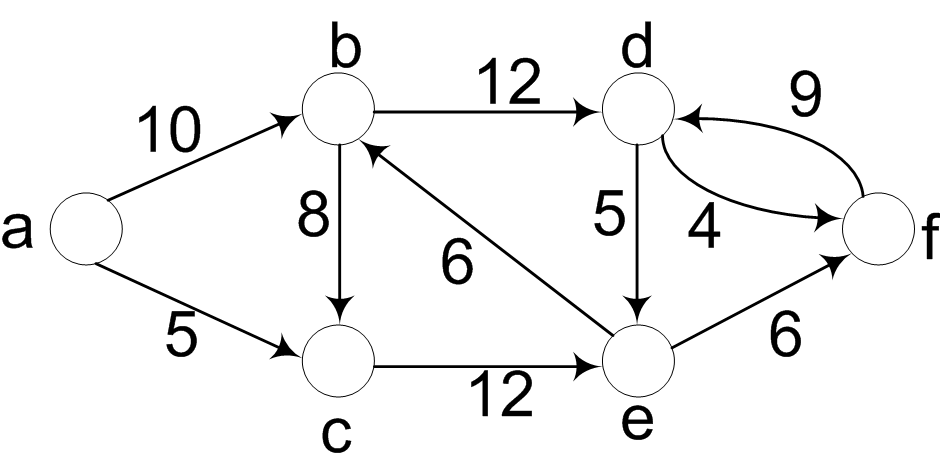
\includegraphics[width=0.5\linewidth]{pics/sp_fig1.png}
	\caption{A directed graph}\label{fig:sp_fig1}
\end{figure}

An example of table is given Table~\ref{tab:example}.
\begin{table}[htb]
	\centering
	\caption{An example of a table}\label{tab:example}
	\begin{tabular}{l|ccccc}
		\toprule
		No of vertices & 64 & 128 & 256 & 384 & 512\\
		\midrule
		Serial &0.1&0.2&0.3&0.4&0.5\\
		Parallel &&&&\\
		Sppedup &2&3&4&5&6\\
		\bottomrule
	\end{tabular}
\end{table} 

\end{document} 

